% F. J. Marshall - J. R. Capablanca, Match, 1909, with Capablanca's notes.
% Build with: python3 ../../tools/chessbook.py game-01-marshall-capablanca.tex
\documentclass[10pt,twoside]{article}
\usepackage[paperwidth=487.56bp,paperheight=691.65bp,top=72pt,bottom=44pt,inner=50pt,outer=48pt,
            headheight=13pt,headsep=20pt,footskip=0pt]{geometry}
\usepackage[T1]{fontenc}
\usepackage[lining]{ebgaramond}
\usepackage{graphicx}
\usepackage{microtype}
\usepackage{tikz}
\usepackage{fancyhdr}
\usepackage[hidelinks,pdftitle={Marshall - Capablanca, Match, 1909},
            pdfauthor={J. R. Capablanca}]{hyperref}

\newcommand{\textsizebook}{\fontsize{10.5}{12.6}\selectfont}
\AtBeginDocument{\textsizebook}
\setlength{\columnsep}{11pt}
\setlength{\parindent}{9pt}
\setlength{\parskip}{0pt}
\setlength{\emergencystretch}{1.5em}
\raggedbottom

\newlength{\boardwidth}
\setlength{\boardwidth}{160pt}

% A main line move, as a bold heading above its note
\newcommand{\Move}[1]{\par\addvspace{8pt}\noindent\phantomsection{\bfseries #1}\par\nopagebreak}
% A diagram in the text
\newcommand{\ChessDiagram}[1]{\par\addvspace{7pt}{\centering #1\par}\addvspace{5pt}}

\pagestyle{fancy}
\fancyhf{}
\renewcommand{\headrulewidth}{0pt}
\fancyhead[LE,RO]{\thepage}
\fancyhead[CE]{Queen's Gambit Declined}
\fancyhead[CO]{Marshall -- Capablanca}





\newcommand{\figK}{\raisebox{-0.14em}{
\includegraphics[height=1em]{diagrams/figK}}}
\newcommand{\figQ}{\raisebox{-0.14em}{
\includegraphics[height=1em]{diagrams/figQ}}}
\newcommand{\figR}{\raisebox{-0.14em}{
\includegraphics[height=1em]{diagrams/figR}}}
\newcommand{\figB}{\raisebox{-0.14em}{
\includegraphics[height=1em]{diagrams/figB}}}
\newcommand{\figN}{\raisebox{-0.14em}{
\includegraphics[height=1em]{diagrams/figN}}}
\begin{document}

\twocolumn[{%
\thispagestyle{empty}
\begin{tikzpicture}[remember picture,overlay]
  \node[circle,draw=black,line width=1.6pt,fill=black!20,minimum size=112pt] (seal)
       at ([xshift=75pt,yshift=-75pt]current page.north west) {};
  \draw[line width=0.9pt] ([shift={(-48pt,-30pt)}]seal.center) -- ([shift={(44pt,34pt)}]seal.center);
  \node[rotate=37] at ([shift={(-11pt,14pt)}]seal.center) {\fontsize{25}{25}\selectfont\bfseries Game};
  \node[rotate=37] at ([shift={(10pt,-16pt)}]seal.center) {\fontsize{38}{38}\selectfont\bfseries 1};
  \node[anchor=north east] at ([xshift=-14pt,yshift=-24pt]current page.north east)
       {\href{https://lichess.org/analysis/pgn/d4_d5_c4_e6_Nc3_Nf6_Bg5_Be7}{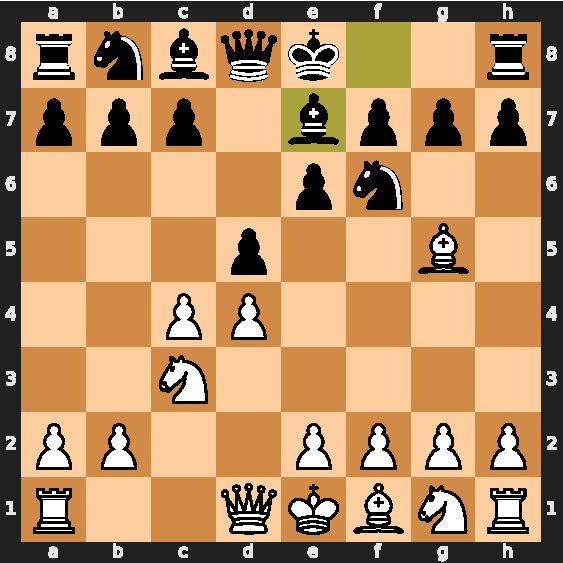
\includegraphics[width=108pt]{diagrams/board-6f3d4b5c56b1}}};
\end{tikzpicture}

\vspace*{38pt}
\begin{center}
  \begin{minipage}{235pt}\centering
    {\fontsize{22}{25}\selectfont\bfseries Queen's Gambit Declined\par}
    \vspace{4pt}\rule{\linewidth}{1pt}\\[-9.5pt]\rule{\linewidth}{0.4pt}
  \end{minipage}

  \vspace{14pt}
  {\fontsize{19}{22}\selectfont\bfseries Marshall -- Capablanca\par}
  \vspace{10pt}
  {\fontsize{15}{18}\selectfont\bfseries Match, 1909\par}
  \vspace{8pt}
  {\fontsize{11}{13}\selectfont White: F. J. Marshall \quad Black: J. R. Capablanca\par}
  \vspace{10pt}
  {\centering\fontsize{8.5}{10}\selectfont\itshape
   Notes by J. R. Capablanca, from \textup{Chess Fundamentals} (1921), which is in the public domain.\\
   Descriptive notation has been converted to algebraic. Page references are to the book.\\
   Click any move or diagram to open it on Lichess.\par}
\end{center}
\vspace{10pt}
}]
\textsizebook

\Move{\href{https://lichess.org/analysis/pgn/d4}{1.d4} \href{https://lichess.org/analysis/pgn/d4_d5}{d5} \href{https://lichess.org/analysis/pgn/d4_d5_c4}{2.c4} \href{https://lichess.org/analysis/pgn/d4_d5_c4_e6}{e6} \href{https://lichess.org/analysis/pgn/d4_d5_c4_e6_Nc3}{3.\figN c3} \href{https://lichess.org/analysis/pgn/d4_d5_c4_e6_Nc3_Nf6}{\figN f6} \href{https://lichess.org/analysis/pgn/d4_d5_c4_e6_Nc3_Nf6_Bg5}{4.\figB g5} \href{https://lichess.org/analysis/pgn/d4_d5_c4_e6_Nc3_Nf6_Bg5_Be7}{\figB e7} \href{https://lichess.org/analysis/pgn/d4_d5_c4_e6_Nc3_Nf6_Bg5_Be7_e3}{5.e3} \href{https://lichess.org/analysis/pgn/d4_d5_c4_e6_Nc3_Nf6_Bg5_Be7_e3_Ne4}{\figN e4}}

I had played this defence twice before in the match with good results, and although I lost this game I still played it until the very last game, when I changed my tactics. The reason was my total lack of knowledge of the different variations in this opening, coupled with the fact that I knew that Dr. E. Lasker had been successful with it against Marshall himself in 1907. I thought that since Dr. Lasker had played it so often, it should be good. The object is to exchange a couple of pieces and at the same time to bring about a position full of possibilities and with promising chances of success once the end-game stage is reached. On general principles it should be wrong, because the same Knight is moved three times in the opening, although it involves the exchange of two pieces. In reality the difficulty in this variation, as well as in nearly all the variations of the Queen's gambit, lies in the slow development of Black's Queen Bishop. However, whether this variation can or cannot be safely played is a question still to be decided, and it is outside the scope of this book. I may add that at present my preference is for a different system of development, but it is not unlikely that I should some time come back to this variation.

\Move{\href{https://lichess.org/analysis/pgn/d4_d5_c4_e6_Nc3_Nf6_Bg5_Be7_e3_Ne4_Bxe7}{6.\figB xe7} \href{https://lichess.org/analysis/pgn/d4_d5_c4_e6_Nc3_Nf6_Bg5_Be7_e3_Ne4_Bxe7_Qxe7}{\figQ xe7} \href{https://lichess.org/analysis/pgn/d4_d5_c4_e6_Nc3_Nf6_Bg5_Be7_e3_Ne4_Bxe7_Qxe7_Bd3}{7.\figB d3}}

\href{https://lichess.org/analysis/pgn/d4_d5_c4_e6_Nc3_Nf6_Bg5_Be7_e3_Ne4_Bxe7_Qxe7_cxd5}{7.cxd5} is preferable for reasons that we shall soon see.

\Move{\href{https://lichess.org/analysis/pgn/d4_d5_c4_e6_Nc3_Nf6_Bg5_Be7_e3_Ne4_Bxe7_Qxe7_Bd3_Nxc3}{7...\figN xc3} \href{https://lichess.org/analysis/pgn/d4_d5_c4_e6_Nc3_Nf6_Bg5_Be7_e3_Ne4_Bxe7_Qxe7_Bd3_Nxc3_bxc3}{8.bxc3} \href{https://lichess.org/analysis/pgn/d4_d5_c4_e6_Nc3_Nf6_Bg5_Be7_e3_Ne4_Bxe7_Qxe7_Bd3_Nxc3_bxc3_Nd7}{\figN d7}}

Now \href{https://lichess.org/analysis/pgn/d4_d5_c4_e6_Nc3_Nf6_Bg5_Be7_e3_Ne4_Bxe7_Qxe7_Bd3_Nxc3_bxc3_dxc4}{8...dxc4} would be a better way to develop the game. The idea is that after \href{https://lichess.org/analysis/pgn/d4_d5_c4_e6_Nc3_Nf6_Bg5_Be7_e3_Ne4_Bxe7_Qxe7_Bd3_Nxc3_bxc3_dxc4}{8...dxc4} \href{https://lichess.org/analysis/pgn/d4_d5_c4_e6_Nc3_Nf6_Bg5_Be7_e3_Ne4_Bxe7_Qxe7_Bd3_Nxc3_bxc3_dxc4_Bxc4}{9.\figB xc4} \href{https://lichess.org/analysis/pgn/d4_d5_c4_e6_Nc3_Nf6_Bg5_Be7_e3_Ne4_Bxe7_Qxe7_Bd3_Nxc3_bxc3_dxc4_Bxc4_b6}{b6}, followed by \figB b7, would give Black's Bishop a powerful range. For this variation see the eleventh game of the match.

\Move{\href{https://lichess.org/analysis/pgn/d4_d5_c4_e6_Nc3_Nf6_Bg5_Be7_e3_Ne4_Bxe7_Qxe7_Bd3_Nxc3_bxc3_Nd7_Nf3}{9.\figN f3} \href{https://lichess.org/analysis/pgn/d4_d5_c4_e6_Nc3_Nf6_Bg5_Be7_e3_Ne4_Bxe7_Qxe7_Bd3_Nxc3_bxc3_Nd7_Nf3_O-O}{0--0}}

No longer would \href{https://lichess.org/analysis/pgn/d4_d5_c4_e6_Nc3_Nf6_Bg5_Be7_e3_Ne4_Bxe7_Qxe7_Bd3_Nxc3_bxc3_Nd7_Nf3_dxc4}{9...dxc4} \href{https://lichess.org/analysis/pgn/d4_d5_c4_e6_Nc3_Nf6_Bg5_Be7_e3_Ne4_Bxe7_Qxe7_Bd3_Nxc3_bxc3_Nd7_Nf3_dxc4_Bxc4}{10.\figB xc4} \href{https://lichess.org/analysis/pgn/d4_d5_c4_e6_Nc3_Nf6_Bg5_Be7_e3_Ne4_Bxe7_Qxe7_Bd3_Nxc3_bxc3_Nd7_Nf3_dxc4_Bxc4_b6}{b6} be good, because \href{https://lichess.org/analysis/pgn/d4_d5_c4_e6_Nc3_Nf6_Bg5_Be7_e3_Ne4_Bxe7_Qxe7_Bd3_Nxc3_bxc3_Nd7_Nf3_dxc4_Bxc4_b6_Bb5}{11.\figB b5} would prevent \figB b7 on account of \figN e5.

\Move{\href{https://lichess.org/analysis/pgn/d4_d5_c4_e6_Nc3_Nf6_Bg5_Be7_e3_Ne4_Bxe7_Qxe7_Bd3_Nxc3_bxc3_Nd7_Nf3_O-O_cxd5}{10.cxd5} \href{https://lichess.org/analysis/pgn/d4_d5_c4_e6_Nc3_Nf6_Bg5_Be7_e3_Ne4_Bxe7_Qxe7_Bd3_Nxc3_bxc3_Nd7_Nf3_O-O_cxd5_exd5}{exd5} \href{https://lichess.org/analysis/pgn/d4_d5_c4_e6_Nc3_Nf6_Bg5_Be7_e3_Ne4_Bxe7_Qxe7_Bd3_Nxc3_bxc3_Nd7_Nf3_O-O_cxd5_exd5_Qb3}{11.\figQ b3} \href{https://lichess.org/analysis/pgn/d4_d5_c4_e6_Nc3_Nf6_Bg5_Be7_e3_Ne4_Bxe7_Qxe7_Bd3_Nxc3_bxc3_Nd7_Nf3_O-O_cxd5_exd5_Qb3_Nf6}{\figN f6} \href{https://lichess.org/analysis/pgn/d4_d5_c4_e6_Nc3_Nf6_Bg5_Be7_e3_Ne4_Bxe7_Qxe7_Bd3_Nxc3_bxc3_Nd7_Nf3_O-O_cxd5_exd5_Qb3_Nf6_a4}{12.a4} \href{https://lichess.org/analysis/pgn/d4_d5_c4_e6_Nc3_Nf6_Bg5_Be7_e3_Ne4_Bxe7_Qxe7_Bd3_Nxc3_bxc3_Nd7_Nf3_O-O_cxd5_exd5_Qb3_Nf6_a4_c5}{c5}}

Played with the intention of obtaining the majority of Pawns on the Queen's side. Yet it is doubtful whether this move is good, since it leaves Black's Queen's-side Pawns disrupted in a way. The safer course would have been to play \href{https://lichess.org/analysis/pgn/d4_d5_c4_e6_Nc3_Nf6_Bg5_Be7_e3_Ne4_Bxe7_Qxe7_Bd3_Nxc3_bxc3_Nd7_Nf3_O-O_cxd5_exd5_Qb3_Nf6_a4_c6}{12...c6}.

\Move{\href{https://lichess.org/analysis/pgn/d4_d5_c4_e6_Nc3_Nf6_Bg5_Be7_e3_Ne4_Bxe7_Qxe7_Bd3_Nxc3_bxc3_Nd7_Nf3_O-O_cxd5_exd5_Qb3_Nf6_a4_c5_Qa3}{13.\figQ a3} \href{https://lichess.org/analysis/pgn/d4_d5_c4_e6_Nc3_Nf6_Bg5_Be7_e3_Ne4_Bxe7_Qxe7_Bd3_Nxc3_bxc3_Nd7_Nf3_O-O_cxd5_exd5_Qb3_Nf6_a4_c5_Qa3_b6}{b6}}

\ChessDiagram{\href{https://lichess.org/analysis/pgn/d4_d5_c4_e6_Nc3_Nf6_Bg5_Be7_e3_Ne4_Bxe7_Qxe7_Bd3_Nxc3_bxc3_Nd7_Nf3_O-O_cxd5_exd5_Qb3_Nf6_a4_c5_Qa3_b6}{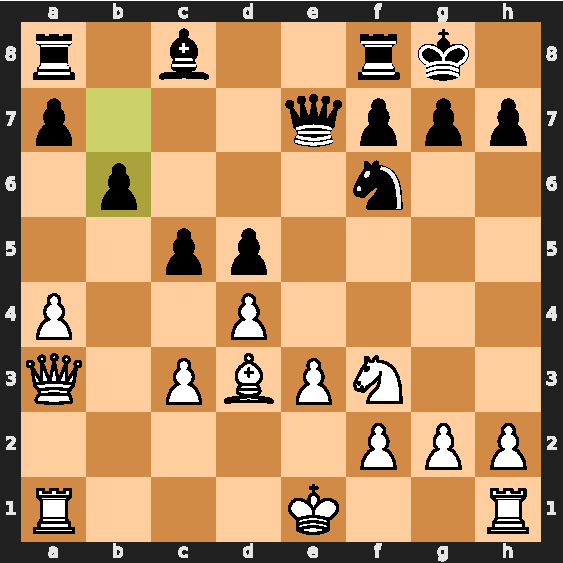
\includegraphics[width=\boardwidth]{diagrams/board-df1e6e933483}}}

This exposes Black to further attack by \href{https://lichess.org/analysis/pgn/d4_d5_c4_e6_Nc3_Nf6_Bg5_Be7_e3_Ne4_Bxe7_Qxe7_Bd3_Nxc3_bxc3_Nd7_Nf3_O-O_cxd5_exd5_Qb3_Nf6_a4_c5_Qa3_b6_a5}{14.a5} without any compensation for it. If I had to play this position nowadays I would simply play \href{https://lichess.org/analysis/pgn/d4_d5_c4_e6_Nc3_Nf6_Bg5_Be7_e3_Ne4_Bxe7_Qxe7_Bd3_Nxc3_bxc3_Nd7_Nf3_O-O_cxd5_exd5_Qb3_Nf6_a4_c5_Qa3_Re8}{13...\figR e8}. Then after \href{https://lichess.org/analysis/pgn/d4_d5_c4_e6_Nc3_Nf6_Bg5_Be7_e3_Ne4_Bxe7_Qxe7_Bd3_Nxc3_bxc3_Nd7_Nf3_O-O_cxd5_exd5_Qb3_Nf6_a4_c5_Qa3_Re8_Qxc5}{14.\figQ xc5} \href{https://lichess.org/analysis/pgn/d4_d5_c4_e6_Nc3_Nf6_Bg5_Be7_e3_Ne4_Bxe7_Qxe7_Bd3_Nxc3_bxc3_Nd7_Nf3_O-O_cxd5_exd5_Qb3_Nf6_a4_c5_Qa3_Re8_Qxc5_Qxc5}{\figQ xc5} would follow, and I believe that Black would regain the Pawn. If, instead, White played \href{https://lichess.org/analysis/pgn/d4_d5_c4_e6_Nc3_Nf6_Bg5_Be7_e3_Ne4_Bxe7_Qxe7_Bd3_Nxc3_bxc3_Nd7_Nf3_O-O_cxd5_exd5_Qb3_Nf6_a4_c5_Qa3_Re8_dxc5}{14.dxc5} then \href{https://lichess.org/analysis/pgn/d4_d5_c4_e6_Nc3_Nf6_Bg5_Be7_e3_Ne4_Bxe7_Qxe7_Bd3_Nxc3_bxc3_Nd7_Nf3_O-O_cxd5_exd5_Qb3_Nf6_a4_c5_Qa3_Re8_dxc5_Bg4}{14...\figB g4} would give Black an excellent game.

\Move{\href{https://lichess.org/analysis/pgn/d4_d5_c4_e6_Nc3_Nf6_Bg5_Be7_e3_Ne4_Bxe7_Qxe7_Bd3_Nxc3_bxc3_Nd7_Nf3_O-O_cxd5_exd5_Qb3_Nf6_a4_c5_Qa3_b6_a5}{14.a5} \href{https://lichess.org/analysis/pgn/d4_d5_c4_e6_Nc3_Nf6_Bg5_Be7_e3_Ne4_Bxe7_Qxe7_Bd3_Nxc3_bxc3_Nd7_Nf3_O-O_cxd5_exd5_Qb3_Nf6_a4_c5_Qa3_b6_a5_Bb7}{\figB b7} \href{https://lichess.org/analysis/pgn/d4_d5_c4_e6_Nc3_Nf6_Bg5_Be7_e3_Ne4_Bxe7_Qxe7_Bd3_Nxc3_bxc3_Nd7_Nf3_O-O_cxd5_exd5_Qb3_Nf6_a4_c5_Qa3_b6_a5_Bb7_O-O}{15.0--0} \href{https://lichess.org/analysis/pgn/d4_d5_c4_e6_Nc3_Nf6_Bg5_Be7_e3_Ne4_Bxe7_Qxe7_Bd3_Nxc3_bxc3_Nd7_Nf3_O-O_cxd5_exd5_Qb3_Nf6_a4_c5_Qa3_b6_a5_Bb7_O-O_Qc7}{\figQ c7} \href{https://lichess.org/analysis/pgn/d4_d5_c4_e6_Nc3_Nf6_Bg5_Be7_e3_Ne4_Bxe7_Qxe7_Bd3_Nxc3_bxc3_Nd7_Nf3_O-O_cxd5_exd5_Qb3_Nf6_a4_c5_Qa3_b6_a5_Bb7_O-O_Qc7_Rfb1}{16.\figR fb1} \href{https://lichess.org/analysis/pgn/d4_d5_c4_e6_Nc3_Nf6_Bg5_Be7_e3_Ne4_Bxe7_Qxe7_Bd3_Nxc3_bxc3_Nd7_Nf3_O-O_cxd5_exd5_Qb3_Nf6_a4_c5_Qa3_b6_a5_Bb7_O-O_Qc7_Rfb1_Nd7}{\figN d7}}

\ChessDiagram{\href{https://lichess.org/analysis/pgn/d4_d5_c4_e6_Nc3_Nf6_Bg5_Be7_e3_Ne4_Bxe7_Qxe7_Bd3_Nxc3_bxc3_Nd7_Nf3_O-O_cxd5_exd5_Qb3_Nf6_a4_c5_Qa3_b6_a5_Bb7_O-O_Qc7_Rfb1_Nd7}{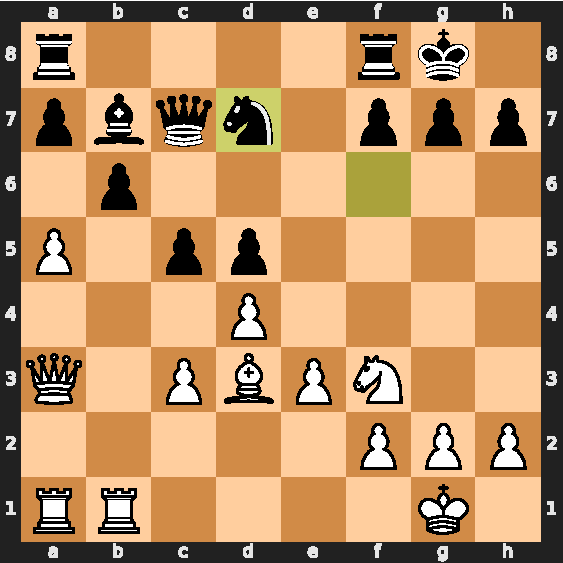
\includegraphics[width=\boardwidth]{diagrams/board-98bb7026b06f}}}

Black's position was bad and perhaps lost in any case, but the text move makes matters worse. As a matter of fact I never saw White's reply \href{https://lichess.org/analysis/pgn/d4_d5_c4_e6_Nc3_Nf6_Bg5_Be7_e3_Ne4_Bxe7_Qxe7_Bd3_Nxc3_bxc3_Nd7_Nf3_O-O_cxd5_exd5_Qb3_Nf6_a4_c5_Qa3_b6_a5_Bb7_O-O_Qc7_Rfb1_Nd7_Bf5}{17.\figB f5}. It never even passed through my mind that this was threatened. Black's best move would have been \href{https://lichess.org/analysis/pgn/d4_d5_c4_e6_Nc3_Nf6_Bg5_Be7_e3_Ne4_Bxe7_Qxe7_Bd3_Nxc3_bxc3_Nd7_Nf3_O-O_cxd5_exd5_Qb3_Nf6_a4_c5_Qa3_b6_a5_Bb7_O-O_Qc7_Rfb1_Rfb8}{16...\figR fb8}. If that loses, then any other move would lose as well.

\Move{\href{https://lichess.org/analysis/pgn/d4_d5_c4_e6_Nc3_Nf6_Bg5_Be7_e3_Ne4_Bxe7_Qxe7_Bd3_Nxc3_bxc3_Nd7_Nf3_O-O_cxd5_exd5_Qb3_Nf6_a4_c5_Qa3_b6_a5_Bb7_O-O_Qc7_Rfb1_Nd7_Bf5}{17.\figB f5} \href{https://lichess.org/analysis/pgn/d4_d5_c4_e6_Nc3_Nf6_Bg5_Be7_e3_Ne4_Bxe7_Qxe7_Bd3_Nxc3_bxc3_Nd7_Nf3_O-O_cxd5_exd5_Qb3_Nf6_a4_c5_Qa3_b6_a5_Bb7_O-O_Qc7_Rfb1_Nd7_Bf5_Rfc8}{\figR fc8}}

From bad to worse. \href{https://lichess.org/analysis/pgn/d4_d5_c4_e6_Nc3_Nf6_Bg5_Be7_e3_Ne4_Bxe7_Qxe7_Bd3_Nxc3_bxc3_Nd7_Nf3_O-O_cxd5_exd5_Qb3_Nf6_a4_c5_Qa3_b6_a5_Bb7_O-O_Qc7_Rfb1_Nd7_Bf5_Nf6}{17...\figN f6} offered the only hope.

\Move{\href{https://lichess.org/analysis/pgn/d4_d5_c4_e6_Nc3_Nf6_Bg5_Be7_e3_Ne4_Bxe7_Qxe7_Bd3_Nxc3_bxc3_Nd7_Nf3_O-O_cxd5_exd5_Qb3_Nf6_a4_c5_Qa3_b6_a5_Bb7_O-O_Qc7_Rfb1_Nd7_Bf5_Rfc8_Bxd7}{18.\figB xd7} \href{https://lichess.org/analysis/pgn/d4_d5_c4_e6_Nc3_Nf6_Bg5_Be7_e3_Ne4_Bxe7_Qxe7_Bd3_Nxc3_bxc3_Nd7_Nf3_O-O_cxd5_exd5_Qb3_Nf6_a4_c5_Qa3_b6_a5_Bb7_O-O_Qc7_Rfb1_Nd7_Bf5_Rfc8_Bxd7_Qxd7}{\figQ xd7} \href{https://lichess.org/analysis/pgn/d4_d5_c4_e6_Nc3_Nf6_Bg5_Be7_e3_Ne4_Bxe7_Qxe7_Bd3_Nxc3_bxc3_Nd7_Nf3_O-O_cxd5_exd5_Qb3_Nf6_a4_c5_Qa3_b6_a5_Bb7_O-O_Qc7_Rfb1_Nd7_Bf5_Rfc8_Bxd7_Qxd7_a6}{19.a6} \href{https://lichess.org/analysis/pgn/d4_d5_c4_e6_Nc3_Nf6_Bg5_Be7_e3_Ne4_Bxe7_Qxe7_Bd3_Nxc3_bxc3_Nd7_Nf3_O-O_cxd5_exd5_Qb3_Nf6_a4_c5_Qa3_b6_a5_Bb7_O-O_Qc7_Rfb1_Nd7_Bf5_Rfc8_Bxd7_Qxd7_a6_Bc6}{\figB c6} \href{https://lichess.org/analysis/pgn/d4_d5_c4_e6_Nc3_Nf6_Bg5_Be7_e3_Ne4_Bxe7_Qxe7_Bd3_Nxc3_bxc3_Nd7_Nf3_O-O_cxd5_exd5_Qb3_Nf6_a4_c5_Qa3_b6_a5_Bb7_O-O_Qc7_Rfb1_Nd7_Bf5_Rfc8_Bxd7_Qxd7_a6_Bc6_dxc5}{20.dxc5} \href{https://lichess.org/analysis/pgn/d4_d5_c4_e6_Nc3_Nf6_Bg5_Be7_e3_Ne4_Bxe7_Qxe7_Bd3_Nxc3_bxc3_Nd7_Nf3_O-O_cxd5_exd5_Qb3_Nf6_a4_c5_Qa3_b6_a5_Bb7_O-O_Qc7_Rfb1_Nd7_Bf5_Rfc8_Bxd7_Qxd7_a6_Bc6_dxc5_bxc5}{bxc5} \href{https://lichess.org/analysis/pgn/d4_d5_c4_e6_Nc3_Nf6_Bg5_Be7_e3_Ne4_Bxe7_Qxe7_Bd3_Nxc3_bxc3_Nd7_Nf3_O-O_cxd5_exd5_Qb3_Nf6_a4_c5_Qa3_b6_a5_Bb7_O-O_Qc7_Rfb1_Nd7_Bf5_Rfc8_Bxd7_Qxd7_a6_Bc6_dxc5_bxc5_Qxc5}{21.\figQ xc5} \href{https://lichess.org/analysis/pgn/d4_d5_c4_e6_Nc3_Nf6_Bg5_Be7_e3_Ne4_Bxe7_Qxe7_Bd3_Nxc3_bxc3_Nd7_Nf3_O-O_cxd5_exd5_Qb3_Nf6_a4_c5_Qa3_b6_a5_Bb7_O-O_Qc7_Rfb1_Nd7_Bf5_Rfc8_Bxd7_Qxd7_a6_Bc6_dxc5_bxc5_Qxc5_Rab8}{\figR ab8}}

The game was lost. One move was as good as another.

\Move{\href{https://lichess.org/analysis/pgn/d4_d5_c4_e6_Nc3_Nf6_Bg5_Be7_e3_Ne4_Bxe7_Qxe7_Bd3_Nxc3_bxc3_Nd7_Nf3_O-O_cxd5_exd5_Qb3_Nf6_a4_c5_Qa3_b6_a5_Bb7_O-O_Qc7_Rfb1_Nd7_Bf5_Rfc8_Bxd7_Qxd7_a6_Bc6_dxc5_bxc5_Qxc5_Rab8_Rxb8}{22.\figR xb8} \href{https://lichess.org/analysis/pgn/d4_d5_c4_e6_Nc3_Nf6_Bg5_Be7_e3_Ne4_Bxe7_Qxe7_Bd3_Nxc3_bxc3_Nd7_Nf3_O-O_cxd5_exd5_Qb3_Nf6_a4_c5_Qa3_b6_a5_Bb7_O-O_Qc7_Rfb1_Nd7_Bf5_Rfc8_Bxd7_Qxd7_a6_Bc6_dxc5_bxc5_Qxc5_Rab8_Rxb8_Rxb8}{\figR xb8} \href{https://lichess.org/analysis/pgn/d4_d5_c4_e6_Nc3_Nf6_Bg5_Be7_e3_Ne4_Bxe7_Qxe7_Bd3_Nxc3_bxc3_Nd7_Nf3_O-O_cxd5_exd5_Qb3_Nf6_a4_c5_Qa3_b6_a5_Bb7_O-O_Qc7_Rfb1_Nd7_Bf5_Rfc8_Bxd7_Qxd7_a6_Bc6_dxc5_bxc5_Qxc5_Rab8_Rxb8_Rxb8_Ne5}{23.\figN e5} \href{https://lichess.org/analysis/pgn/d4_d5_c4_e6_Nc3_Nf6_Bg5_Be7_e3_Ne4_Bxe7_Qxe7_Bd3_Nxc3_bxc3_Nd7_Nf3_O-O_cxd5_exd5_Qb3_Nf6_a4_c5_Qa3_b6_a5_Bb7_O-O_Qc7_Rfb1_Nd7_Bf5_Rfc8_Bxd7_Qxd7_a6_Bc6_dxc5_bxc5_Qxc5_Rab8_Rxb8_Rxb8_Ne5_Qf5}{\figQ f5} \href{https://lichess.org/analysis/pgn/d4_d5_c4_e6_Nc3_Nf6_Bg5_Be7_e3_Ne4_Bxe7_Qxe7_Bd3_Nxc3_bxc3_Nd7_Nf3_O-O_cxd5_exd5_Qb3_Nf6_a4_c5_Qa3_b6_a5_Bb7_O-O_Qc7_Rfb1_Nd7_Bf5_Rfc8_Bxd7_Qxd7_a6_Bc6_dxc5_bxc5_Qxc5_Rab8_Rxb8_Rxb8_Ne5_Qf5_f4}{24.f4} \href{https://lichess.org/analysis/pgn/d4_d5_c4_e6_Nc3_Nf6_Bg5_Be7_e3_Ne4_Bxe7_Qxe7_Bd3_Nxc3_bxc3_Nd7_Nf3_O-O_cxd5_exd5_Qb3_Nf6_a4_c5_Qa3_b6_a5_Bb7_O-O_Qc7_Rfb1_Nd7_Bf5_Rfc8_Bxd7_Qxd7_a6_Bc6_dxc5_bxc5_Qxc5_Rab8_Rxb8_Rxb8_Ne5_Qf5_f4_Rb6}{\figR b6} \href{https://lichess.org/analysis/pgn/d4_d5_c4_e6_Nc3_Nf6_Bg5_Be7_e3_Ne4_Bxe7_Qxe7_Bd3_Nxc3_bxc3_Nd7_Nf3_O-O_cxd5_exd5_Qb3_Nf6_a4_c5_Qa3_b6_a5_Bb7_O-O_Qc7_Rfb1_Nd7_Bf5_Rfc8_Bxd7_Qxd7_a6_Bc6_dxc5_bxc5_Qxc5_Rab8_Rxb8_Rxb8_Ne5_Qf5_f4_Rb6_Qxb6}{25.\figQ xb6!}}

\noindent\textbf{Resigns.}

Of course, if \href{https://lichess.org/analysis/pgn/d4_d5_c4_e6_Nc3_Nf6_Bg5_Be7_e3_Ne4_Bxe7_Qxe7_Bd3_Nxc3_bxc3_Nd7_Nf3_O-O_cxd5_exd5_Qb3_Nf6_a4_c5_Qa3_b6_a5_Bb7_O-O_Qc7_Rfb1_Nd7_Bf5_Rfc8_Bxd7_Qxd7_a6_Bc6_dxc5_bxc5_Qxc5_Rab8_Rxb8_Rxb8_Ne5_Qf5_f4_Rb6_Nxc6}{25.\figN xc6} \href{https://lichess.org/analysis/pgn/d4_d5_c4_e6_Nc3_Nf6_Bg5_Be7_e3_Ne4_Bxe7_Qxe7_Bd3_Nxc3_bxc3_Nd7_Nf3_O-O_cxd5_exd5_Qb3_Nf6_a4_c5_Qa3_b6_a5_Bb7_O-O_Qc7_Rfb1_Nd7_Bf5_Rfc8_Bxd7_Qxd7_a6_Bc6_dxc5_bxc5_Qxc5_Rab8_Rxb8_Rxb8_Ne5_Qf5_f4_Rb6_Nxc6_Rb1}{\figR b1+} would have drawn. The text move is pretty and finishes quickly. A well-played game on Marshall's part.

\end{document}
